%% DONE
\id{МРНТИ 65.29.03}{}

\begin{articleheader}
\sectionwithauthors{М.Н. Рахымбаева, А.И. Истаев, Т.К. Кулажанов, М.А. Якияева, Ш.А. Турсунбаева}{ҚАЗАҚСТАНДАҒЫ АСЫЛ ТҰҚЫМДЫ ҚЫСТЫҚ ЖӘНЕ ЖАЗДЫҚ БИДАЙ СҰРЫПТАРЫНЫҢ РЕОЛОГИЯЛЫҚ ЖӘНЕ НАН ПІСІРУ ҚАСИЕТТЕРІН ЗЕРТТЕУ}

{\bfseries
М.Н. Рахымбаева\authorid,
А.И. Изтаев\authorid,
Т.К. Кулажанов\authorid,
М.А. Якияева\textsuperscript{\envelope } \authorid,
Ш.А. Турсунбаева\authorid}
\end{articleheader}

\begin{affiliation}
\emph{Aлмaты тeхнологиялық унивepcитeтi, Aлмaты қ., Қaзaқcтaн,}

\raggedright \textsuperscript{\envelope }{\em Корреспондент-автор: \href{mailto:yamadina88@mail.}{\nolinkurl{yamadina88@mail.}}ru}
\end{affiliation}

Мақалада отандық әртүрлі жаздық және күздік бидай сұрыптарының
реологиялық және нандық сапа көрсеткіштері бойынша зерттеу деректері
келтірілген. Зерттеу нысаны отандық жаздық бидай сұрыптары: Алмекен
элита, Казахстанская раннеспелая, Казахстанская 10, Егемен, Мереке.
Күздік бидай сұрыптары: Стекловидная 24,Сапалы, Богарная 56, Степная 75,
Алмакен болды. Бұл жұмыстың мақсаты альвеограф пен Mixolabты қолдана
отырып, отандық жаздық және күздік бидай сұрыптары дәнінен жасалған
ұнның реологиялық қасиеттерін зерттеу болды. Зерттеу жүргізу үшін бидай
үлгілері келесідей нөмірленді: № 1 -- Жұмсақ жаздық бидай «Казахстанская
10», № 2 -- Жұмсақ жаздық бидай «Алмекен элита», № 3 -- Жұмсақ жаздық
бидай «Казахстанская раннеспелая», № 4 -- Жұмсақ жаздық бидай « Егемен»,
№ 5 -- Жұмсақ жаздық бидай «Мереке», № 6 -- Күздік бидай «Сапалы», № 7
-- Күздік бидай «Стекловидная 24», № 8 -- Күздік бидай «Богарная 56», №
9 -- Күздік бидай «Степная 75», № 10 -- Күздік бидай «Алмакен». Отандық
жаздық және күздік жұмсақ бидай сұрыптары Қазақстан Республикасының Ауыл
шаруашылығы министрлігі шешімімен өндірісте қолдануға рұқсат берілген.
Егіс даласында бұл сұрыптар егіліп өнім алынып жатыр. Сапалы нандық
сұрыптарын алу үшін олардың қамырының реологиялық қасиеттерін тереңірек
заманауи Mixolab және Альвеограф аспабында зерттеліп, қамырларынан
стандартты нандарын жасап, реологиялық және нандық қасиеттерінің
көрсеткіштерінің арасындағы байланыстары анықталды. Осы анықталған
байланыстардың негізінде жұмсақ бидай сұрыптарын аудан, аумақ көлемінде
ұтымды ұндық партияларын қалыптастырып, үлкен көлемде сапалы ұн
сұрыптарын алудың технологиялық ұсыныстары қабылданады. Осыған сәйкес
қамырдың серпімділігі, қамырдың созылуы, серпімділіктің созылғыштыққа
қатынасы, қамырдың деформациясының жұмысы, ісіну индексі, жұмсақ
ортасының ылғалдылығы, жұмсақ ортасының қышқылдылығы, кеуектілігі,
сыртқы түрі, беті, жұмсақ ортасының жағдайы, жұмсақ ортасының түсі
көрсеткіштері анықталды. Сынақтың ең үлкен созылуы жұмсақ жаздық бидай
«Казахстанская 10», күздік бидай «Сапалы», күздік бидай «Степная 75»,
сұрыпында анықталды және 85 құрады. Алынған нәтижелерді талдау
көрсеткендей, жұмсақ жаздық бидай «Казахстанская 10» - қамыр
деформациясының нақты энергиясы бойынша 219 болды. Қамырдың стандартты
реологиялық қасиетімен салыстырсақ (280) күшті ұн болып саналады.

{\bfseries Түйын cөздep:} қамыр, біртұтас тартылған жұмсақ бидай ұны, нан
өнімдерінің сапалық көрсеткіштері, ұн сапасы.

\begin{articleheader}
{\bfseries ИССЛЕДОВАНИЕ РЕОЛОГИЧЕСКИХ И ХЛЕБОПЕКАРНЫХ СВОЙСТВ ПЕРСПЕКТИВНЫХ СОРТОВ ОЗИМОЙ И ЯРОВОЙ ПШЕНИЦЫ В КАЗАХСТАНЕ}

{\bfseries
М.Н. Рахымбаева,
А.И. Изтаев,
Т.К. Кулажанов,
М.А. Якияева\textsuperscript{\envelope },
Ш.А. Турсунбаева}
\end{articleheader}

\begin{affiliation}
\emph{Aлмaтинcкий тeхнологичecкий унивepcитeт, г. Aлмaты, Кaзaхcтaн,}

\emph{e-mail: \href{mailto:yamadina88@mail.}{\nolinkurl{yamadina88@mail.}}ru}
\end{affiliation}

В статье представлены результаты исследований реологических и
хлебопекарных показателей качества различных отечественных сортов яровой
и озимой пшеницы. Объектом исследования стали отечественные сорта яровой
пшеницы: Алмекен элита, Казахстанская раннеспелая, Казахстанская 10,
Егемен, Мереке. Озимые сорта пшеницы: Стекловидная 24, Сапалы, Богарная
56, Степная 75, Алмакен. Цель работы -- изучение реологических свойств
муки, полученной из зерна отечественных сортов яровой и озимой пшеницы,
с использованием альвеографа и Mixolab. Для проведения исследования
образцы пшеницы были пронумерованы следующим образом:№ 1 -- мягкая
яровая пшеница «Казахстанская 10», № 2 -- мягкая яровая пшеница «Алмекен
элита», № 3 -- мягкая яровая пшеница «Казахстанская раннеспелая», № 4 --
мягкая яровая пшеница «Егемен», № 5 -- мягкая яровая пшеница «Мереке», №
6 -- озимая пшеница «Сапалы», № 7 -- озимая пшеница «Стекловидная 24», №
8 -- озимая пшеница «Богарная 56», № 9 -- озимая пшеница «Степная 75», №
10 -- озимая пшеница «Алмакен». Отечественные сорта яровой и озимой
мягкой пшеницы разрешены к использованию в производстве по решению
Министерства сельского хозяйства Республики Казахстан. Эти сорта засеяны
на полях и дают урожай. Для получения качественного хлеба исследованы
реологические свойства теста с использованием современных приборов
Mixolab и альвеографа. Созданы стандартные образцы хлеба из теста,
выявлены связи между реологическими показателями теста и хлебопекарными
свойствами. На основе этих данных разрабатываются технологические
рекомендации по производству качественной муки в больших объемах, с
формированием рациональных партий в пределах региона или территории
произрастания мягкой пшеницы. В ходе исследования определены следующие
показатели: эластичность теста, растяжимость теста, соотношение
эластичности к растяжимости, работа деформации теста, индекс набухания,
влажность, кислотность, пористость, внешний вид, состояние и цвет
мякиша. Наибольшая растяжимость теста выявлена у сортов мягкой яровой
пшеницы «Казахстанская 10», озимой пшеницы «Сапалы» и озимой пшеницы
«Степная 75», составив 85 мм. Анализ результатов показал, что мягкая
яровая пшеница «Казахстанская 10» имеет фактическую энергию деформации
теста 219 ЕД. По сравнению со стандартными реологическими свойствами
теста (280 ЕД) она относится к муке с повышенной крепостью.

{\bfseries Ключeвыe cловa:} Тесто, цельномолотая мука мягкой пшеницы,
качественные показатели хлебобулочных изделий, качество муки.

\begin{articleheader}
{\bfseries STUDY OF RHEOLOGICAL AND BAKING PROPERTIES OF PROMISING WINTER AND SPRING WHEAT VARIETIES IN KAZAKHSTAN}

{\bfseries
M.N.Rakhimbayeva,
A.I.Iztayev,
T.K.Kulazhanov,
M.A.Yakiyayevа\textsuperscript{\envelope },
Sh.A. Tursunbayeva}
\end{articleheader}

\begin{affiliation}
\emph{Almaty Technological University, Almaty, Kazakhstan,}

\emph{e-mail: \href{mailto:yamadina88@mail.}{\nolinkurl{yamadina88@mail.}}ru}
\end{affiliation}

The article presents the results of studies on the rheological and
baking quality indicators of various domestic varieties of spring and
winter wheat. The research objects were domestic varieties of spring
wheat: Almeken Elite, Kazakhstan Early Maturing, Kazakhstan 10, Egemen,
and Mereke. Winter wheat varieties: Steklovidnaya 24, Sapaly, Bogarnaya
56, Stepnaya 75, and Almaken. The aim of the study was to examine the
rheological properties of flour obtained from domestic varieties of
spring and winter wheat using an alveograph and Mixolab. For the study,
wheat samples were numbered as follows: No. 1 -- soft spring wheat
"Kazakhstan 10", No. 2 -- soft spring wheat "Almeken Elite", No. 3 --
soft spring wheat "Kazakhstan Early Maturing", No. 4 -- soft spring
wheat "Egemen", No. 5 -- soft spring wheat "Mereke", No. 6 -- winter
wheat "Sapaly", No. 7 -- winter wheat "Steklovidnaya 24", No. 8 --
winter wheat "Bogarnaya 56", No. 9 -- winter wheat "Stepnaya 75", No. 10
-- winter wheat "Almaken". Domestic varieties of soft spring and winter
wheat are approved for use in production by the decision of the Ministry
of Agriculture of the Republic of Kazakhstan. These varieties are sown
in fields and produce yields. To obtain high-quality bread, the
rheological properties of the dough were studied using modern devices
such as Mixolab and an alveograph. Standard bread samples were created
from the dough, and correlations between the rheological indicators of
the dough and the baking properties of the bread were identified. Based
on these findings, technological recommendations are being developed for
producing high-quality flour in large volumes, with the formation of
rational batches within the region or territory where soft wheat is
grown. During the study, the following parameters were determined: dough
elasticity, dough extensibility, elasticity-to-extensibility ratio,
dough deformation energy, swelling index, moisture content, acidity,
porosity, appearance, texture and crumb color. The highest dough
extensibility was observed in soft spring wheat "Kazakhstan 10", winter
wheat "Sapaly", and winter wheat "Stepnaya 75", reaching 85 mm. Analysis
of the results showed that soft spring wheat "Kazakhstan 10" has an
actual dough deformation energy of 219 EU. Compared to the standard
rheological properties of dough (280 EU), it is classified as flour with
increased strength.

{\bfseries Keywords:} Dough, whole-ground soft wheat flour, quality
indicators of bakery products, flour quality..

\begin{multicols}{2}
{\bfseries Кіріспе.} Ұндық және нандық қасиеттері жоғарғы сападағы жаздық
және күздік жұмсақ сұрыптарынан биологиялық және тағамдық құндылығы
тағам өнімін өндіруде, оның негізгі шикізаты ретінде ұнның өзіндік
қасиеттеріне және құрамына ұтымды өзгерістері болуы тиіс {[}1{]}.Осындай
өзгерістері бар ұн ол 70\% шығымы бар біркелкі толық тартылған
дәндерінен алынған өнім.

Бұл біркелкі 70\% шығымы бар тартылған бидай ұндарын алудың сандық және
сапалық көрсеткіштерінің талаптарына сәйкес технологиялық жүйесі
құрастырылды.

Майдаланатын жұмсақ бидай дәндері толық ішіндегі қоспалардан
тазартылады, іріліктері бір деңгейге келтіріледі, ылғалдылығы бір орта
шамаға жеткізіледі W=13,5-14,0 \% {[}2{]}. Оның физикалық және химиялық
көрсеткіштері базистік шамада болуы тиіс. Осындай сападағы бидай ұнын
мамандандырылған LabMill- зертханалық диірменде тартылған біркелкі 70\%
шығымы бар нандық ұндарын аламыз.

Осы алынған біркелкі ұндардың стандартты нандық жоғарғы, бірінші, екінші
және 72\% бірінші сұрыптармен салыстырғанда барлық көрсеткіштері бойынша
айырмашылықтары бар екенін тәжірбиелер нәтижелері көрсетті.

Бұл біркелкі 70\% шығымы бар ұндардан 19-20\% бөлігі кебек ретінде
бөлініп негізгі стандартты ұн сұрыптарына қосылмайды. Ол майдаланған
кебек ұнтағында кейбір витаминдер, белок компоненттері, клечатка
талшықтар, макро және микро элементтері өте көп орыналасқан {[}3{]}.

Біркелкі 70\% шығымы бар тартылған бидай ұндары енді ғана толық жаңа
сұрыптар бойынша зерттеліп келеді. Біздің ғылыми жұмысымызда денсаулыққа
пайдалы жаңа отандық жұмсақ бидай сұрыптарынан біркелкі 70\% шығымы бар
тартылған ұн және нан өнімдерін алуды бірінші рет қарастырып отыр. Жақсы
нан өнімдерін алудың технологиясын жасауда, ілгерілі бидай сұрыптарының
реологиялық және нандық қасиеттерін зерттеудің ғылыми және практикалық
тұрғыдан маңыздылығы өте зор.

Соңғы жылдары ұнның реологиялық қасиеттерін зерттеу ұн сапасын
бағалаудың маңызды бағыты ретінде дамып келеді. Ұнның реологиялық
сипаттамалары нан-тоқаш өнімдерінің құрылымы мен консистенциясына
тікелей әсер етеді. Зерттеулер көрсеткендей, ұнның реологиялық
қасиеттерін жақсарту үшін түрлі ферменттік және белсенді қоспалар
қолданылады {[}4{]}. Сонымен қатар, нан пісіру технологияларында ұн
құрамын модификациялау арқылы өнімнің сапасын арттыру бойынша
эксперименттер жүргізілуде {[}5{]}.

Нан пісіру саласындағы заманауи зерттеулер нан өнімдерінің құрылымын
жақсарту және сақтау мерзімін ұзарту мақсатында ұн құрамындағы ақуыз,
крахмал және ферменттік жүйелердің өзара әрекеттесуін талдауға
негізделген. Мысалы, нанотехнологияларды қолдану арқылы глютен желісінің
беріктігін арттыру және нан өнімдерінің сапасын тұрақтандыруға мүмкіндік
бар {[}6{]}. Сондай-ақ, нанобөлшектер қосылған ұнды пайдалану өнімнің
қоректік құндылығын жақсартуға ықпал етеді {[}7{]}.

Жаздық және күздік жұмсақ бидай астығының көрсеткіштері, илеу үдерісінде
қамырдың (реологиялық қасиеттері), шамалардың өзгеруіне әкеледі {[}8{]}.

{\bfseries Материалдар мен әдістер.} Бұл зерттеуде жұмсақ жаздық және
күздік бидай пайдаланылды. Зерттеу нысандары ретінде Отандық жаздық
бидай сұрыптары: Алмекен элита, Казахстанская раннеспелая, Казахстанская
10, Егемен, Мереке және күздік бидай сұыптары: Стекловидная 24,Сапалы,
Богарная 56, Степная 75, Алмакен алынды.

Ұнның сапасын МЕМСТ 9404-60 стандартты тәсілі бойынша тексерілді. МЕМСТ
9404-60 стандартына сәйкес желімшенің сапасы оның серпімділігі,
созылғыштығы және түсі бойынша көзмөлшермен бағаланды. Желімшенің
созылғыштығы I (жақсы), II (орташа) және III (нашар) деп үш топқа
бөлінді {[}10{]}.

Қамырдың физикалық қасиеттерін альвеограф көмегімен зерттелді.
Альвеограф ұнның наубайханалық күшін бағалайды. Бұл көрсеткіш қамырдың
белгілі бір мөлшердегі жұқа жайылған қабаты астына ауа үрлеп, шар
тәрізді желқабық пайда болғанша үрлеу арқылы анықталды. Желқабық
жарылған кезде жұмсалған жұмыс мөлшері қамырдың беріктігін сипаттады.
Альвеографта (МЕМСТ 51415-99 (ИСО 5530-4-91) бойынша) келесі
көрсеткіштер зерттелді:

- қамырдың серпімділігі (P);

- қамырдың созылғыштығы (L);

- серпімділіктің созылғыштыққа қатынасы (P/L);

- қамырдың деформация энергиясы (W) -- ұнның беріктігін сипаттайтын
жалпылама көрсеткіш.

Қамырдың реологиялық қасиеттерін Mixolab құрылғысында зерттелді. Mixolab
көмегімен:

- ұнның суды сіңіру қабілеті;

- қамыр илеу ұзақтығы;

- глютен мөлшері;

- қамырдың тұтқырлығы;

- амилаза мөлшері;

- ретроградация деңгейі анықталды {[}11{]}.

Наның иісі мен түсі қолданылған шикізатгың кұрамы мен қасиетіне,
қамырдың ашуына, пісуіне байланысты Нанның иісі мен түсіне нанды сақтау
жағдайлары да әсерін тигізеді. Ашу үдерісінде қамырдың құрамында этил
спирті, органикалық қышқыл, эфирлер жиналады, әрине оларда нанның иісі
мен түсіне өз әсерін тигізеді.

Нанның сапасы МЕМСТ 5667-65 «Нан және нан-тоқаш өнімдері. Өнімді
қабылдау, үлгі алу және органолептикалық көрсеткіштерді анықтау әдісі»
бойынша бағаланды. Нанның сапасы төмендегі көрсеткіштер бойынша
зерттелді:

- сыртқы түрі (формасы, бетінің сапасы);

- жұмсақ ортасының құрылымы (кеуектілігі, біртектілігі);

- түсі (қызғылт реңі, біркелкілігі);

- дәмі мен иісі (ашыту процесіне байланысты өзгерістері);

- ылғалдылық деңгейі (36-39\%);

- қышқылдылығы (0,4-0,8 град);

- кеуектілік коэффициенті (44-59\%) {[}12{]}.

Қамырда серпімділік, созылғыштық, беріктік, түтқырлық, түсетін күшке
релаксациялық қабілеті бар реологиялық қасиет үйлестірілген. Қамырдың
реологиялық қасиеті бірінші кезекте үнның күшіне, сондай-ақ әртүрлі
технологиялық: температура, ылғалдылық, илеу кезіндегі механикалық
әрекет етудің ұзақтығы және қарқындылығы, рецептура, қамыр дайындау
әдісімен ашу үзактығы, ұнның наубайханалық қасиетіне және т.б.
факторларға байланысты {[}13,14{]}.

Қамырдың реологиялық қасиеттерін анықтау үшін «Шопен» фирмасының
альвеографы қолданылды. Бұл құрылғы қамырдың серпімділігі, созылғыштығы
және беріктігін бағалауға мүмкіндік береді. Зерттеу барысында қамыр
үлгісінің ауа қысымына қарсылығы өлшеніп, алынған деректер кимограф
барабанына жазылады. Нәтижесінде алынған альвеограмма қисық сызығы
қамырдың наубайханалық қасиеттерін сипаттайды.

Зерттеу әдісі

1. Қамыр дайындау:

- сынама 2,5\%-дық ас тұзы ерітіндісімен ұннан дайындалды;

- ұн мен ерітіндінің қатынасы 250 г ұнға 125 мл ерітінді (ылғалдылық --
14,3\%) деңгейінде алынды;

- қамырдың температурасы 25°C болуы қадағаланды.

2. Қамырды илеу:

- илеу 6 минутқа созылды;

- дайын қамыр арнайы қабылдағыш құрылғы арқылы стандартты қалыпқа
келтірілді;

- термостаттау: қалыпқа келтірілген қамыр дискісі альвеографтың
25°C-тағы термостатында 26 минут бойы тұрақтандырылды.

3. Сынақ жүргізу:

- қамыр үлгісі альвеограф құрылғысында ауа ағынымен үрленіп, оның
жұқалығы мен беріктігі тексерілді;

- туындаған ауа қысымы кимограф барабанындағы қағазға қисық сызық
(альвеограмма) ретінде тіркелді.

Қамырдың серпімділігі мен беріктігі жоғарылаған сайын, оның
наубайханалық қасиеттері жақсарады. Альвеографиялық зерттеу нәтижелері
қамырдың сапасын анықтауға және наубайханалық өндірістегі ұнның
тиімділігін бағалауға мүмкіндік береді {[}15,16{]}.

Альвеограммада қамырдың серпімділігі (P -- максимальды артық қысым, мм),
созылымдылығы (L -- үзілу кезіндегі абсциссаның орташа мәні, мм),
олардың қатынасы (P/L), қамырдың үзілуі үшін созылу шығынына кететін
қамыр деформациясының энергиясы (W--10⁻⁴ J/г) анықталады. Ұн күші жоғары
болған сайын, оның P және W шамалары да артады.

Альвеографта (МЕМСТ 51415-99 (ИСО 5530-4-91) бойынша) қамырдың
реологиялық қасиеттерін зерттеу үшін келесі көрсеткіштер анықталды:

- қамырдың серпімділігі (P) -- қамырдың қарсылық күші мен иілгіштігін
сипаттайды;

- серпімділіктің созылуға қатынасы (P/L) -- қамырдың механикалық
тұрақтылығын бағалау үшін қолданылады;

- қамырдың деформациялық энергиясы (W) -- қамырдың беріктігін
сипаттайтын кешенді көрсеткіш;

Зерттеу әдісі:

1. Қамыр дайындау: сынамалар 2,5\%-дық ас тұзы ерітіндісімен иленген
қамырдан жүргізілді. Ұнның ылғалдылығы 14,3\% болған жағдайда 250 г
ұнға 125 мл тұз ерітіндісі қолданылды.

2. Температуралық бақылау: қамырдың температурасы 25°C деңгейінде
сақталды.

3. Қамырды илеу: 6 минут бойы жүргізілді, содан кейін қамыр арнайы
қалыптау құрылғысы арқылы стандартты үлгіге келтірілді.

4. Термостаттау: дайын қамыр үлгілері 25°C температурада 26 минут бойы
термостатта сақталды.

5. Сынақ жүргізу: қамыр үлгісі альвеограф құрылғысында үрленіп, оның
жұқалығы мен беріктігі өлшенді.

6. Қисық сызықты талдау: алынған альвеограмма көмегімен қамырдың
серпімділік, беріктік және созылымдылық көрсеткіштері анықталды.

Қамырдың қасиеттерін бағалау алынған диаграммалар арқылы жүргізілді. Бұл
әдіс ұнның сапасын дәл бағалауға мүмкіндік береді және наубайханалық
қасиеттерді болжауға негіз болады {[}19{]}.

Ұнның суды сіңіру қабілеті, қамыр илеу ұзақтығы, глютен мөлшері,
қамырдың тұтқырлығы, амилаза мөлшері, ретроградация миксолаб аппаратында
зерттелді.

{\bfseries Нәтижелер және талқылау.} Бұл зерттеулерде біртұтас жұмсақ
жаздық және күздік бидай сұрыптарыны ұндарының және дайын өнімдердің
реологиялық қасиеттері стандарттарға сәйкес анықталды.

Жаздық және күздік бидай сұрыптарының 70\%-тік ұндарынан алынған
қамырының альвеограммалық көрсеткіштері бойынша нәтижелері 1-- суретте
берілген.

1-суреттегі берілген бидай сұрыптарының көрсеткіштері бойынша талдау
жасалынып сұрыптардың өздеріне байланысты жекешеленген мынадай
сипаттамасын талдаймыз.

1-суреттен көріп отырғанымыздай, сынақтың ең үлкен серпімділігі Жұмсақ
жаздық бидай «Алмакен», сұрыпында анықталды және 148 мм болды, ал бұл
сынақтың созылуы 37 мм болды. Жұмсақ жаздық бидай «Казахстанская 10»
сұрыпының бидайынан жасалған қамырдың серпімділігі 54 мм, ал созылуы 140
мм болды.
\end{multicols}

\begin{figure}[H]
	\centering
	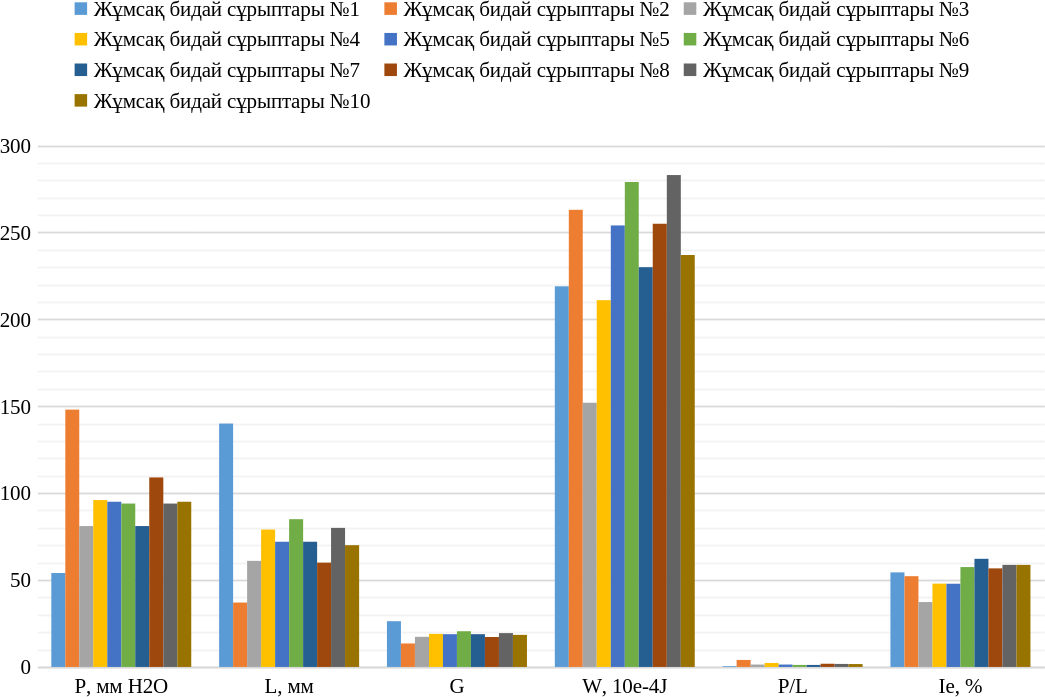
\includegraphics[width=0.9\textwidth]{media/pish2/image29}
	\caption*{1 - сурет. Бидай сұрыптарының 70\%-тік ұндарынан алынған қамырының альвеограммалық көрсеткіштері}
\end{figure}

\begin{figure}[H]
	\centering
	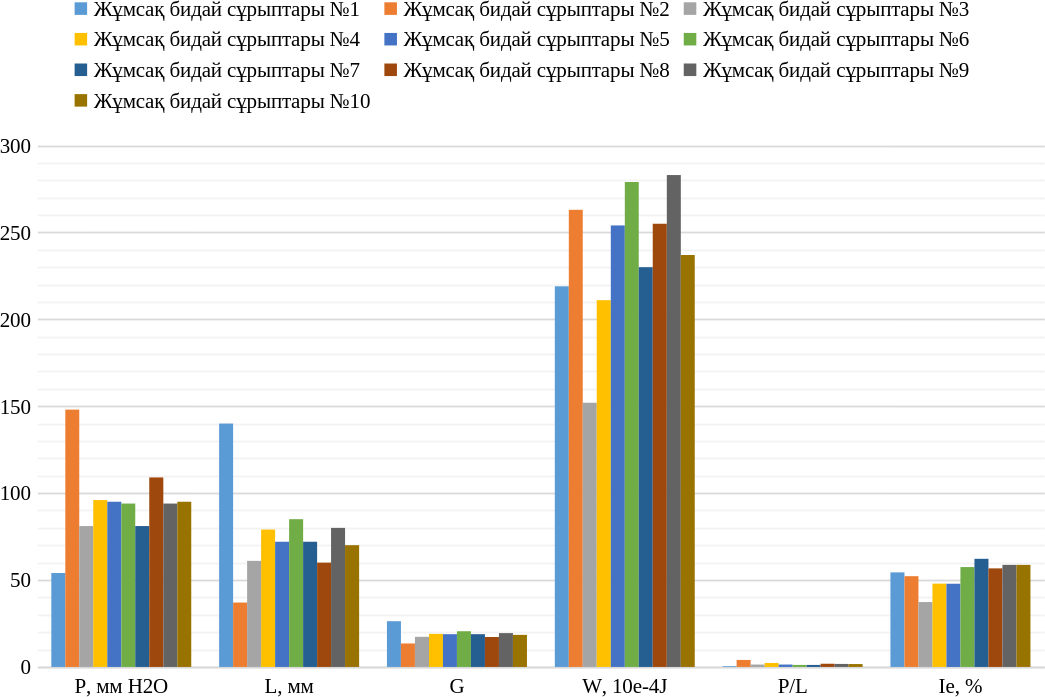
\includegraphics[width=0.9\textwidth]{media/pish2/image29}
	\caption*{2 - сурет. Бидай сұрыптарының 70\%-тік ұндарынан алынған қамырының Mixolab көрсеткіштері}
\end{figure}

\begin{multicols}{2}
Серпімділіктің созылғыштығына қатынасы сұрыптар бойынша 0,39-1,82
аралығында болды. Күздік бидай «Богарная 56» бидай сұрыпында жоғары
мөлшерде болды.

Қамырдың деформациясының нақты энергиясы бойынша 152-283 аралығында
болды. Күздік бидай «Степная 75», күздік бидай «Сапалы» және жаздық
бидай «Алмекен», сұрыптарында жоғары болды.

Жұмсақ жаздық бидай «Казахстанская 10» және күздік бидай «Степная 75»
сұрыптарын жоғары сапалы нан өнімдерін өндіруде пайдалану үшін ең жоғары
көрсеткіштерге ие, дегенмен барлық басқа сұрыптар нан өнімдерінің
сапасына қойылатын талаптарға сәйкес келеді.

2-суретте бидай сұрыптарының 70\%-тік ұндарынан алынған қамырының
Mixolab көрсеткіштері берілген.

2-суретте келтірілген деректер зерттелетін жұмсақ бидай сорттарының
Mixolab сынағының реологиялық қасиеттері кең ауқымда өзгеретінін
көрсетеді. Сонымен, қамырдың су сіңіру қабілеті бойынша жұмсақ жаздық
бидай «Казахстанская раннеспелая» сұрыпында 62,1\% жоғары болды. Ең аз
мөлшерде жұмсақ жаздық бидай «Казахстанская 10», жұмсақ жаздық бидай
«Алмекен» сұрыптарында 57,0 \%. Глютен мөлшері бойынша жұмсақ жаздық
бидай «Алмекен» сұрыпында 8, жұмсақ жаздық бидай «Казахстанская 10»
сұрыпында 2 болды. Қамырдың тұтқырлығы бойынша жұмсақ жаздық бидай
«Алмекен» сұрыпында жоғары 6 мөлшерінде, жұмсақ жаздық бидай
«Казахстанская раннеспелая» сұрыпында 3 болды. Амилаза мөлшері жұмсақ
жаздық бидай «Алмекен» сұрыпында жоғары 8, ретроградация шамасында
жұмсақ жаздық бидай «Алмекен», жұмсақ жаздық бидай «Казахстанская
раннеспелая», жұмсақ жаздық бидай «Мереке», күздік бидай «Богарная 56» 7
шамасында болды. Ең аз көрсеткіш жұмсақ жаздық бидай «Казахстанская 10»
болды.

Осылайша, зерттелетін күздік және жаздық жұмсақ бидай сұрыптарының
реологиялық қасиеттерін зерттеу олардың барлығы дерлік жұмсақ бидай
сұрыптарына қойылатын талаптарға жауап беретінін, бидай сапасының
көрсеткіштерінің мәні әртүрлілікке байланысты өзгеретінін көрсетті.

Жаздық және күздік жұмсақ бидай ұны нан өнімдерінің сапалық
көрсеткіштері бойынша нәтижелері 1-кестеде берілген
\end{multicols}

\begin{longtblr}[
  label = none,
  entry = none,
  caption = {\bfseries 1 - кесте Біртұтас тартылған жұмсақ бидай ұны нан өнімдерінің сапалық көрсеткіштері},
]{
  colspec = {X[0.2] X[1] X[1] X[1] X[0.5] X[1] X[1] X[1.5] X[1]},
  row{1} = {c},
  row{2} = {c},
  cell{1}{1} = {c=9}{},
  cell{3}{1} = {c},
  cell{3}{3} = {c},
  cell{3}{4} = {c},
  cell{3}{5} = {c},
  cell{4}{1} = {c},
  cell{4}{3} = {c},
  cell{4}{4} = {c},
  cell{4}{5} = {c},
  cell{4}{6} = {r=10}{},
  cell{4}{7} = {r=10}{},
  cell{4}{9} = {r=10}{},
  cell{5}{1} = {c},
  cell{5}{3} = {c},
  cell{5}{4} = {c},
  cell{5}{5} = {c},
  cell{6}{1} = {c},
  cell{6}{3} = {c},
  cell{6}{4} = {c},
  cell{6}{5} = {c},
  cell{7}{1} = {c},
  cell{7}{3} = {c},
  cell{7}{4} = {c},
  cell{7}{5} = {c},
  cell{8}{1} = {c},
  cell{8}{3} = {c},
  cell{8}{4} = {c},
  cell{8}{5} = {c},
  cell{9}{1} = {c},
  cell{9}{3} = {c},
  cell{9}{4} = {c},
  cell{9}{5} = {c},
  cell{9}{8} = {r=5}{},
  cell{10}{1} = {c},
  cell{10}{3} = {c},
  cell{10}{4} = {c},
  cell{10}{5} = {c},
  cell{11}{1} = {c},
  cell{11}{3} = {c},
  cell{11}{4} = {c},
  cell{11}{5} = {c},
  cell{12}{1} = {c},
  cell{12}{3} = {c},
  cell{12}{4} = {c},
  cell{12}{5} = {c},
  cell{13}{1} = {c},
  cell{13}{3} = {c},
  cell{13}{4} = {c},
  cell{13}{5} = {c},
  vlines,
  hlines,
}
Көрсеткіштердің атауы &                 &                                  &                                   &                &                  &                                           &                                                                                                 &                                      \\
№                     & Бидай сұрыптары & Жұмсақ ортасының ылғалдылығы, \% & Жұмсақ ортасының қышқылдығы, град & Кеуек тілік, \% & Сыртқы түрі:     & Беті                                      & Жұмсақ ортасының жағдайы                                                                        & Жұмсақ ортасының түсі                \\
1                     & Бақылау үлгісі  & 35                               & 0,7                               & 44             & Нанның өзіне тән & Тегіс, үлкен жарықтар мен жарықшақтар жоқ & Газды ұстау қабілеті жақсы және нанның көтерілу күші пішіні тұрақты                             & Ақшыл-сары түсі нанға сәйкес келеді  \\
2                     & №1              & 32                               & 0,8                               & 59             & Нанның өзіне тән & Тегіс, үлкен жарықтар мен жарықшақтар жоқ & Газды ұстау қабілеті жақсы және нанның көтерілу күші пішіні тұрақты                             & Ақшыл-сары түсті нанға сәйкес келеді \\
3                     & №2              & 39                               & 0,4                               & 46             &                  &                                           & Газ түзетін және газ ұстау қабілеті әлсіз тұрақтылық жоқ                                        &                                      \\
4                     & №3              & 38                               & 0,8                               & 47             &                  &                                           & Газ түзуші қабілеті бар газ ұстаушы қабілеті әлсіз, расстойкада қамырда көпіршіктер пайда болды &                                      \\
5                     & №4              & 36                               & 0,6                               & 46             &                  &                                           & Газды ұстау қабілеті тұрақты емес                                                               &                                      \\
6                     & №5              & 36                               & 0,7                               & 45             &                  &                                           & Газ түзетін және газ ұстайтын қабілеті орташа                                                   &                                      \\
7                     & №6              & 36                               & 0,6                               & 51             &                  &                                           & Газ түзетін және газ ұстайтын қабілеті тұрақты көтерілу күші жақсы                              &                                      \\
8                     & №7              & 38                               & 0,4                               & 40             &                  &                                           &                                                                                                 &                                      \\
9                     & №8              & 37                               & 0,6                               & 44             &                  &                                           &                                                                                                 &                                      \\
10                    & №9              & 37                               & 0,5                               & 46             &                  &                                           &                                                                                                 &                                      \\
11                    & №10             & 36                               & 0,4                               & 46             &                  &                                           &                                                                                                 &                                      
\end{longtblr}

\begin{multicols}{2}
1-кестеден көріп отырғанымыздай бақылау үлгісінің ылғалдылығы 35\%,
қышқылдығы 0,7 град, кеуектілігі 44 \%, ісі өзіне тән, беті тегіс, үлкен
жарықтар мен жарықшақтар жоқ, жұмсақ ортасының жағдайы бойынша газды
ұстау қабілеті жақсы және нанның көтерілу күші пішіні тұрақты, және
жұмсақ ортасының түсі ақшыл-сары түсті нанға сәйкес келді. Зерттеу
үлгілерінен жасалған нан өнімдерінің жұмсақ ортасының ылғалдылығы 32-39
\% ие болды. Жұмсақ ортасының қышқылдылығы 0,4-0,8 град аралығында
болды. Кеуектілігі 40-59 \% болды. Нанның сыртқы түрі өзіне тән иісі
бар. Беті тегіс, үлкен жарықтар мен жарықшақтар жоқ. Жұмсақ ортасының
жағдайы Жұмсақ жаздық бидай «Казахстанская 10» сұрыпында газды ұстау
қабілеті жақсы және нанның көтерілу күші пішіні тұрақты. Күздік бидай
«Стекловидная 24» сұрыпында газ түзетін және газ ұстайтын қабілеті
орташа, түсі орташа. Күздік бидай «Богарная 56» сұрыпында газ түзетін
және газ ұстайтын қабілеті тұрақты көтерілу күші жақсы,түсі нанға сәйкес
келеді. Жаздық және күздік бидай сұрыптары бойынша Күздік бидай
«Стекловидная 24», күздік бидай «Богарная 56», жұмсақ жаздық бидай
«Казахстанская 10» нандық қасиеттері жоғары болды. Бақылау үлгісімен
салыстырғанда №1, №6-№10 үлгілер жоғары нәтиже көрсетті, оның ішінде №1
үлгінің кеуектілігі және жұмсақ ортасының жағдайы жақсы нәтиже көрсетті
және бақылау үлгісімен салыстырганда жоғары болды.

Қазақстан -- әлемдегі ірі астық экспорттаушы елдердің бірі, сондықтан
бидайдың сапалық көрсеткіштері елдің азық-түлік қауіпсіздігі мен
экспорттық әлеуеті үшін өте маңызды. Асыл тұқымды қыстық және жаздық
бидай сұрыптарының реологиялық және нан пісіру қасиеттерін зерттеу ұн
сапасын бағалауға, жоғары сапалы нан өнімдерін шығаруға және ауыл
шаруашылығы өндірісінің тиімділігін арттыруға мүмкіндік береді. Бұл
зерттеулер нан өнімдерінің технологиялық қасиеттерін жақсартуға,
экологиялық жағдайларға төзімді сұрыптарды іріктеуге және Қазақстанның
астық өнімдерін халықаралық нарықта бәсекеге қабілетті етуге ықпал
етеді.

Зерттеу нәтижелері:

- селекциялық жұмыстарды дамытуға көмектеседі, яғни нан пісіруге жарамды
жоғары сапалы бидай сұрыптарын шығару мүмкін болады;

- астықты қайта өңдеу саласында қолданылып, диеталық және функционалдық
қасиеттері жақсартылған нан өнімдерін жасауға мүмкіндік береді;

- экспорттық саясатты жетілдіруге ықпал етеді, себебі жоғары сапалы ұн
мен бидай сұрыптары шетел нарығында сұранысқа ие болады;

- нан өндірісінің тиімділігін арттырады, себебі бидайдың нан пісіру
қасиеттері жақсы болған сайын, өнімнің сапасы мен сақтау мерзімі де
жоғарылайды.

Бұл зерттеулер Қазақстанның ауыл шаруашылығы мен тамақ өнеркәсібінің
тұрақты дамуына және әлемдік нарықта өз орнын нығайтуға маңызды үлес
қосады.

Бұл зерттеу Қазақстанда өсірілетін жаздық және күздік жұмсақ бидай
сұрыптарының ерекшеліктерін ғылыми тұрғыдан дәлелдеуге бағытталған.
Аймақтық климаттық жағдайлар мен топырақ ерекшеліктері ескеріліп,
отандық сұрыптардың реологиялық және нан пісіру қасиеттеріне нақты баға
берілді. Жұмыста Chopin фирмасының Альвеограф және Mixolab құрылғылары
бірге пайдаланылды. Бұл екі құрылғының кешенді қолданылуы бидай
қамырының серпімділігі, созылғыштығы, деформация энергиясы және
тұтқырлығы туралы толыққанды деректер алуға мүмкіндік берді. Жанама
зерттеулерде көбінесе жаздық және күздік бидай сұрыптары жеке
қарастырылса, бұл зерттеу олардың аралас ұн партияларын құру мүмкіндігін
көрсетіп, ұн зауыттарында өндіріс тиімділігін арттыру жолдарын ұсынды.
Бұл отандық астық өңдеу саласында маңызды практикалық нәтиже болып
табылады. Яғни, жаздық және күздік бидайдан алынған ұндар сапасы бойынша
айтарлықтай айырмашылық көрсетпей, тұрақты нан пісіру қасиеттерін
сақтайтыны дәлелденді. Бұл зерттеудің нәтижелері өндірістік деңгейде
тексеріліп, ұн тарту кәсіпорындары мен наубайханалар үшін тәжірибелік
маңызы жоғары екендігі көрсетілді. Осы ерекшеліктердің барлығы зерттеуді
отандық ауыл шаруашылығы мен тамақ өнеркәсібі үшін аса маңызды,
өндірісте қолдануға бағытталған қолданбалы зерттеу ретінде ерекшелейді.

{\bfseries Қорытынды.} Зерттеу нәтижелері Қазақстанда өсірілетін жаздық
және күздік жұмсақ бидай сұрыптарының реологиялық қасиеттерінің өзара
ұқсастықтары мен ерекшеліктерін ғылыми тұрғыдан дәлелдеуге мүмкіндік
берді. 10 түрлі сұрыптың ұндарының реологиялық қасиеттері Chopin
фирмасының Альвеограф және Mixolab құрылғылары арқылы зерттеліп,
қамырдың серпімділігі, созылғыштығы және деформация энергиясы бойынша
көрсеткіштері анықталды. Жаздық бидай сұрыптарында серпімділік жоғары
(148 мм), ал күздік бидай сұрыптарында бұл көрсеткіш 109 мм-ге дейін
төмендейтіні байқалды. Mixolab құрылғысының нәтижелері де екі бидай
түрінің реологиялық қасиеттерінде ұқсастықтар бар екенін көрсетті.
Сонымен қатар, Алмекен элита сұрыпы глютен мөлшері мен тұтқырлығы
бойынша айтарлықтай ерекшеленді. Зерттеу нәтижелері ұн зауыттарында
жаздық және күздік бидай сұрыптарын біріктіріп, ұн партияларын
қалыптастыру мүмкіндігін дәлелдеді. Бұл астық өңдеу саласында өндірістік
тиімділікті арттырып, ұнның сапалық тұрақтылығын қамтамасыз етуге ықпал
етеді. Дайын нан өнімдерінің сапа көрсеткіштері бір деңгейде екені
анықталды: жұмсақ ортасының ылғалдылығы -- 36-39\%, ортасының
қышқылдылығы -- 0,4-0,8 град, кеуектілігі -- 44-59\%. Барлық сұрыптар
бойынша нанның органолептикалық көрсеткіштері (сыртқы түрі, бетінің
сапасы, жұмсақ ортасының құрылымы, түсі) бірдей деңгейде болды. Болашақ
зерттеулердің бағыттары:

- климаттың өзгеруіне бейімделген сұрыптарды шығару: әртүрлі экологиялық
жағдайларда бидай сұрыптарының тұрақтылығын зерттеу және олардың
өнімділігін арттыру;

- нан өнімдерінің сапасын жақсарту: қоспаларды қолдану арқылы нан пісіру
қасиеттерін жақсарту және жаңа технологияларды енгізу;

- ұн өндірісінде автоматтандыру мен жаңа технологияларды енгізу: ұн
сапасын тұрақтандыру үшін интеллектуалды жүйелерді қолдану;

- генетикалық және биотехнологиялық зерттеулер: жоғары сапалы,
функционалды және тағамдық құндылығы жоғары бидай сұрыптарын дамыту.

Бұл зерттеулер Қазақстанның ауыл шаруашылығы мен тамақ өнеркәсібінің
тұрақты дамуына ықпал етіп, экспорттық әлеуетін арттыруға көмектеседі.
\end{multicols}

\begin{center}
{\bfseries Әдибиеттер}
\end{center}

\begin{references}
1. Винчевский М.А., Храпко О.П. Роль сорта в формировании качества муки
// Молодые исследователи агропромышленного и лесного комплексов --
регионам: сборник материалов III международной молодежной
научно-практической конференции. Вологда, 2018. -С. 6-12.

2. Волюшин Е.В. Зерноведение с основами растениеводства: учебное пособие.
-- Оренбург, 2019. - 97 с. ISBN 978-5-7410-2420-1

3. Цыбикова Г.Ц. Основы технологии производства продуктов питания из
растительного сырья: учебное пособие. - Изд. Лань, 2021.- 92 с. ISBN
978-5-8114-3051-2

4. Rosell C. M., Rojas J. A., Benedito de Barber C. Influence of
hydrocolloids on dough rheology and bread quality//Food Hydrocolloids.-
2019. -Vol. 32(1)- P.132-140.

\href{https://doi.org/10.1016/s0268-005x(00)00054-0}{DOI
10.1016/s0268-005x(00)00054-0}

5. Cauvain S. P., Young L. S. Technology of Breadmaking. - 3rd ed. -
Springer, 2020. - 380 p.

6. Gómez M., Jiménez S., Ruiz E., Oliete B. Effect of fiber addition on
the quality of dough and bread // Journal of Cereal Science.- 2003.
-Vol. 216(1) - С. 51-56. DOI 10.1007/s00217-002-0632-9

7. Wang J.,Rosell C.M., Benedito de Barber C. Effect of the addition of
different fibres on wheat dough performance and bread guality//Food
Chemistry.-2002.-Vol.79(2).-P.221-226. DOI \\10.1016/s0308-8146(02)00135-8

8. Оспанов Ә.Ә., Муслимов Н.Ж., Тимурбекова А.Қ., Жұмабекова Г.Б. Көп
дәнді өнімдерді өндіру технологиясы: оқу құралы. - Алматы: «Нур Принт»,
2015. - 120. ISBN 978-601-7390-87-7

9. Белкина Р.И. Факторы повышения качества зерна пшеницы в условиях
Северного Зауралья// Зерновые культуры. -1999.- № 6.- С.16 -- 18

10. Маликгаева П.М., Сексенбаева Ж.М., Шымыр Ж.А. Нан өндірісінің
технологиясы : оқу құралы / П.М.Маликтаева, Ж.М.Сексенбаева, Ж.А.Шымыр-
Алматы : Эпиграф, 2022. - 176 с. -{\bfseries ~}ISBN~978-601-652-538-9

11. Мармузова Л.В. Нан пісіру өндірісінің технологиясы. Шикізат және
материалдар: оқу құралы. - Мәскеу: Академия, 2015. - 288 б. ISBN 978-601-333-055-06

12. Кулеватова Т.Б., Лящева С.В., Злобина Л.Н., Старичкова Н.И. К
качеству зерна озимой пшеницы // Изв. Сарат. ун-та. Нов. Сер. Химия.
Биология. Экология.- 2021.-Т.21(1)-С. 78-86. DOI\\
10.18500/1816-9775-2021-21-1-78-86

13. Мелешкина Е.П., Коломиец С.Н., Жильцова Н.С., Бундина О.И.
Современная оценка хлебопекарных свойств российской пшеницы // Вестник
Воронежского государственного университета инженерных технологий.-
2021.- Т. 83(1) - С. 155-162.
\href{https://doi.org/10.20914/2310-1202-2021-1-155-162}{DOI
10.20914/2310-1202-2021-1-155-162}

14. Винчевский М.А., Храпко О.П. Роль сорта в формировании качества муки
// Молодые исследователи агропромышленного и лесного комплексов -
регионам: сборник материалов III международной молодежной
научно-практической конференции.- Вологда, 2018. - С.6-12.

15. Байысбаева М.П. Нан өнімдерінің технологиясы:оқулық. -Алматы: Эверо,
2020.- 354 б. ISBN 978-601-327-419-5

16. Смирнова В.В., Сидельникова Н.А., Шмайлова Т.А. Качество зерна
различных сортов озимой пшеницы // Научное обеспечение инновационного
развития агропромышленного комплекса регионов РФ: сборник материалов
международной научно-практической конференции. - Курган, 2018. - С.
644-648.

17. Ушаков Т.И., Чиркова Л.В. Овес и продукты его переработки
//Хлебопродукты.- 2015.- № 11.- С. 49-51.

18. Туляков Д.Г., Мелешкина Е.П., Витол И.С., Панкратов Г.Н., Кандроков
Р.Х. Оценка свойств муки из зерна тритикале с использованием системы
Миксолаб // Хранение и переработка сельхозсырья. -- 2017. -- № 1. -- С.
20-23.

19. Бурчакова И.Ю., Ермилова С.В. Организация процесса приготовления и
приготовление сложных хлебобулочных, мучных кондитерских изделий.
Учебник -2-е изд.-Москва:Академия, 2015.-383 с. ISBN 978-5-4468-2134-1
\end{references}

\begin{center}
{\bfseries References}
\end{center}

\begin{references}
1. Vinchevskij M.A., Hrapko O.P. Rol'{} sorta v
formirovanii kachestva muki // Molodye issledovateli agropromyshlennogo
i lesnogo kompleksov -regionam: sbornik materialov III mezhdunarodnoj\\
molodezhnoj nauchno-prakticheskoj konferencii. Vologda, 2018. -S. 6-12.
{[}in Russuan{]}

2. Voljushin E.V. Zernovedenie s osnovami rastenievodstva: uchebnoe
posobie. -- Orenburg, 2019. - 97 s. ISBN 978-5-7410-2420-1.{[}in
Russuan{]}

3. Cybikova G.C. Osnovy tehnologii proizvodstva produktov pitanija iz
rastitel' nogo syr' ja: uchebnoe posobie.
- Izd. Lan', 2021.- 92 s. ISBN 978-5-8114-3051-2. {[}in
Russuan{]}

4. Rosell C. M., Rojas J. A., Benedito de Barber C. Influence of
hydrocolloids on dough rheology and bread quality//Food Hydrocolloids.-
2019. -Vol. 32(1)- P.132-140.

\href{https://doi.org/10.1016/s0268-005x(00)00054-0}{DOI
10.1016/s0268-005x(00)00054-0}

5. Cauvain S. P., Young L. S. Technology of Breadmaking. - 3rd ed. -
Springer, 2020. - 380 p.

6. Gómez M., Jiménez S., Ruiz E., Oliete B. Effect of fiber addition on
the quality of dough and bread // Journal of Cereal Science.- 2003.
-Vol. 216(1) - С. 51-56. DOI 10.1007/s00217-002-0632-9

7. Wang J.,Rosell C.M., Benedito de Barber C. Effect of the addition of
different fibres on wheat dough performance and bread guality//Food
Chemistry.-2002.-Vol.79(2).-P.221-226. DOI \\10.1016/s0308-8146(02)00135-8

8. Ospanov Ә.Ә., Muslimov N.Zh., Timurbekova A.Қ., Zhұmabekova G.B. Kөp
dәndі өnіmderdі өndіru tehnologijasy: oқu құraly. - Almaty: «Nur Print»,
2015. - 120. ISBN 978-601-7390-87-7. {[}in Kazakh{]}

9. Belkina R.I. Faktory povyshenija kachestva zerna pshenicy v uslovijah
Severnogo Zaural' ja// Zernovye kul' tury.
-1999.- № 6.- S.16 -- 18.{[}in Russian{]}

10. Malikgaeva P.M., Seksenbaeva Zh.M., Shymyr Zh.A. Nan өndіrіsіnің
tehnologijasy : oқu құraly / P.M.Maliktaeva, Zh.M.Seksenbaeva,
Zh.A.Shymyr- Almaty : Jepigraf, 2022. - 176 s. - ISBN 978-601-652-538-9.
{[}in Kazakh{]}

11. Marmuzova L.V. Nan pіsіru өndіrіsіnің tehnologijasy. Shikіzat zhәne
materialdar:

oқu құraly. - Mәskeu: Akademija, 2015. - 288 b. ISBN 978-601-333-055-06.
{[}in Kazakh{]}

12. Kulevatova T.B., Ljashheva S.V., Zlobina L.N., Starichkova N.I. K
kachestvu zerna ozimoj pshenicy // Izv. Sarat. un-ta. Nov. Ser. Himija.
Biologija. Jekologija.- 2021.-T.21(1)-S. 78-86. DOI
10.18500/1816-9775-2021-21-1-78-86. {[}in Russian{]}

13. Meleshkina E.P., Kolomiec S.N., Zhil' cova N.S.,
Bundina O.I. Sovremennaja ocenka hlebopekarnyh svojstv rossijskoj
pshenicy // Vestnik Voronezhskogo gosudarstvennogo universiteta
inzhenernyh \\tehnologij.- 2021.- T. 83(1) - S. 155-162.
DOI 10.20914/2310-1202-2021-1-155-162. {[}in Russian{]}

14. Vinchevskij M.A., Hrapko O.P. Rol'{} sorta v
formirovanii kachestva muki // Molodye issledovateli agropromyshlennogo
i lesnogo kompleksov - regionam: sbornik materialov III mezhdunarodnoj\\
molodezhnoj nauchno-prakticheskoj konferencii.- Vologda, 2018. - S.6-12.
{[}in Russian{]}

15. Bajysbaeva M.P. Nan өnіmderіnің tehnologijasy:oқulyқ. -Almaty:
Jevero, 2020.- 354 b. ISBN 978-601-327-419-5. {[}in Kazakh{]}

16. Smirnova V.V., Sidel' nikova N.A., Shmajlova T.A.
Kachestvo zerna razlichnyh sortov ozimoj pshenicy // Nauchnoe
obespechenie innovacionnogo razvitija agropromyshlennogo kompleksa
regionov RF: sbornik materialov mezhdunarodnoj nauchno-prakticheskoj
konferencii. - Kurgan, 2018. - S. 644-648. {[}in Russian{]}

17. Ushakov T.I., Chirkova L.V. Oves i produkty ego pererabotki
//Hleboprodukty.- 2015.- № 11.- S. 49-51. {[}in Russian{]}

18. Tuljakov D.G., Meleshkina E.P., Vitol I.S., Pankratov G.N.,
Kandrokov R.H. Ocenka svojstv muki iz zerna tritikale s
ispol' zovaniem sistemy Miksolab // Hranenie i
pererabotka sel' hozsyr' ja. -2017. - № 1.
- S. 20-23. {[}in Russian{]}

19. Burchakova I.Ju., Ermilova S.V. Organizacija processa prigotovlenija
i prigotovlenie slozhnyh \\hlebobulochnyh, muchnyh konditerskih izdelij.
Uchebnik -2-e izd.-Moskva:Akademija, 2015.-383 s. ISBN
978-5-4468-2134-1. {[}in Russian{]}
\end{references}

\begin{authorinfo}
\emph{{\bfseries Сведения об авторах}}

Рахымбаева М.Н. - магистр, докторант, Алматы технологиялық университеті,
Алматы, Қазақстан, e-mail:\\
\href{mailto:m.r.n_8704@mail.ru}{\nolinkurl{m.r.n\_8704@mail.ru}};

Изтаев F.-техникалық ғылымдар докторы, профессор, ҚР ҰҒА академигі,
Алматы технологиялық университеті, Алматы, Қазақстан,
e-mail:\href{mailto:auelbekking@mail.ru}{\nolinkurl{auelbekking@mail.ru}};

Кулажанов Т.К.- техникалық ғылымдар докторы, профессор, ҚР ҰҒА
академигі, Алматы технологиялық университеті, Алматы, Қазақстан,
e-mail:\href{mailto:tkulazhanov_atu@mail.ru}{\nolinkurl{tkulazhanov\_atu@mail.ru}};

Якияева М.А. - философия докторы (Ph.D), қауымдастырылған профессор,
Алматы технологиялық университеті, Алматы, Қазақстан,
e-mail:\href{mailto:yamadina88@mail.ru}{\nolinkurl{yamadina88@mail.ru}};

Турсунбаева Ш. А. - философия докторы (Ph.D), Алматы технологиялық
университеті, Алматы, Қазақстан, e-mail:
\href{mailto:sh.tursunbaeva@bk.ru}{\nolinkurl{sh.tursunbaeva@bk.ru}}

\emph{{\bfseries Information about authors}}

Rakhymbayeva M. N.-Master's degree holder, PhD student, Almaty
University of Technology, Almaty, Kazakhstan, e-mail:
\href{mailto:m.r.n_8704@mail.ru}{\nolinkurl{m.r.n\_8704@mail.ru}};\\
Iztayev A. -Doctor of Technical Sciences, Professor, Academician of the
National Academy of Sciences of the Republic of Kazakhstan, Almaty
University of Technology, Almaty, Kazakhstan, e-mail:
\href{mailto:auelbekking@mail.ru}{\nolinkurl{auelbekking@mail.ru}};\\
Kulazhanov T.K. {\bfseries -} Doctor of Technical Sciences, Professor,
Academician of the National Academy of Sciences of the Republic of
Kazakhstan, Almaty University of Technology, Almaty, Kazakhstan, e-mail:
\href{mailto:tkulazhanov_atu@mail.ru}{\nolinkurl{tkulazhanov\_atu@mail.ru}};\\
Yakiyayeva M. A{\bfseries .} - Doctor of Philosophy (Ph.D), Associate
Professor, Almaty University of Technology, Almaty, Kazakhstan,e-mail:
\href{mailto:yamadina88@mail.ru}{\nolinkurl{yamadina88@mail.ru}};\\
Tursunbayeva Sh.A.-

Doctor of Philosophy (Ph.D), Almaty University of Technology, Almaty,
Kazakhstan, e-mail:
\href{mailto:sh.tursunbaeva@bk.ru}{\nolinkurl{sh.tursunbaeva@bk.ru}}
\end{authorinfo}
